\documentclass[accentcolor=tud7b,noresetcounter]{tudbeamer}

\usepackage[ngerman]{babel}
\usepackage[utf8]{inputenc}
\usepackage[T1]{fontenc}

% footmisc behebt u.a. Probleme mit Fu?noten in Abschnittstiteln
\usepackage[stable]{footmisc}

% Einbinden von Grafiken erm?glichen
\usepackage{graphicx}

% Paket xtab erm?glicht Umbrechen von langen Tabellen
\usepackage{xtab}
\usepackage{tikz}

% picins erlaubt das Umflie?en von Abbildungen durch Text
% Untenstehendes renewcommand behebt den picins-bug, dass Abbildungen
% nicht im Abbildungsverzeichnis auftauchen
%\usepackage{picins}
\makeatletter
%\renewcommand\piccaption{\@dblarg{\@piccaption}}
\makeatother

\usepackage{verbatim}

% Paket setspace erlaubt Umschalten auf 1.5fachen Zeilenabstand
\usepackage{setspace}

\usepackage{hyperref}
\usepackage{listings}
\usepackage{amssymb}
\usepackage{newclude}
\usepackage{multirow}
\usepackage{array}
\usepackage{tabularx}
\usepackage{hyperref} 
\usepackage{graphicx}
\usepackage{pgfplots}
\usepackage{csvsimple}
%Erm?glicht Hyperlinks zwischen Textstellen und zu externen Dokumenten
%% breaklinks=true/false: Gibt an, ob Links umgebrochen werden d?rfen.
%% linktocpage=true/false: im Inhaltsverzeichnis sind nur die Seitenzahlen
%% links, nicht der Text
%% colorlinks=true/false: Links werden eingef?rbt (Farben werden mit
%% linkcolor, anchorcolor \dots festgelegt)
%% linkcolor=Farbe: Farbe des verlinkten Textes, Dokument-interne Links
%% citecolor=Farbe: Farbe des verlinkten Textes, Links zum
%% Literaturverzeichnis
%% filecolor=Farbe: Farbe des verlinkten Textes, Links auf lokale Dateien
%% urlcolor=Farbe: Farbe des verlinkten Textes, externe URLs
%% frenchlinks=true/false: Links werden als smallcaps, anstatt farbig
%% dargestellt.
%% breaklinks=true/false: Gibt an, ob Links umgebrochen werden d?rfen.
\hypersetup{%
  linktocpage=true,
  breaklinks=true,
  colorlinks=true,
  citecolor=black,
  urlcolor=black,
  linkcolor=black,
  pdfpagemode=UseThumbs,
  pdftitle=Übung 2 - Webmining,
  pdfauthor=Ingo Adrian und Steffen Pegenau,
  pdfsubject=Webmining,
  %pdfkeywords=xy
}


\lstset{ %
  %backgroundcolor=\color{white},   % choose the background color; you must add 
%\usepackage{color} or \usepackage{xcolor}
  %basicstyle=\footnotesize,        % the size of the fonts that are used for 
					%the code
  %breakatwhitespace=false,         % sets if automatic breaks should only 
%happen at whitespace
  breaklines=true,                 % sets automatic line breaking
  %captionpos=b,                    % sets the caption-position to bottom
  commentstyle=\bf,    % comment style
  %deletekeywords={...},            % if you want to delete keywords from the 
%given language
  %escapeinside={\%*}{*)},          % if you want to add LaTeX within your code
  %extendedchars=true,              % lets you use non-ASCII characters; for 
%8-bits encodings only, does not work with UTF-8
  frame=single,                    % adds a frame around the code
  %keepspaces=true,                 % keeps spaces in text, useful for keeping 
%indentation of code (possibly needs columns=flexible)
  %keywordstyle=\color{blue},       % keyword style
  language=html,                 % the language of the code
  %otherkeywords={*,...},            % if you want to add more keywords to the 
%set
  numbers=left,                    % where to put the line-numbers; possible 
%values are (none, left, right)
  %numbersep=5pt,                   % how far the line-numbers are from the code
  %numberstyle=\tiny\color{mygray}, % the style that is used for the 
%line-numbers
  %rulecolor=\color{black},         % if not set, the frame-color may be 
changed 
%on line-breaks within not-black text (e.g. comments (green here))
  %showspaces=false,                % show spaces everywhere adding particular 
%underscores; it overrides 'showstringspaces'
  %showstringspaces=false,          % underline spaces within strings only
  %showtabs=false,                  % show tabs within strings adding 
particular 
%underscores
  %stepnumber=2,                    % the step between two line-numbers. If 
it's 
%1, each line will be numbered
  %stringstyle=\color{mymauve},     % string literal style
  tabsize=4,                       % sets default tabsize to 2 spaces
  %title=\lstname                   % show the filename of files included with 
%\lstinputlisting; also try caption instead of title
}

% bibtex
%\usepackage[backend=biblatex]{biblatex}

%\bibliography{refs}
%\addbibresource{refs.bib}

%%%%%%%%%%%%%%%%%%%%%%%%%%%%%%%%%%%%%%%%%%%%%%%%%%%%%%%%%%%%%%%%%%%%%%%%%%%%%%%%%%%%%%

\title%[Klima \& Geographie] % (optional, only for long titles)
{Web Mining: Übung 2}
\subtitle{Lösungsvorschlag}

\author[Ingo Adrian und Steffen Pegenau]{}
\institute[Fachbereich Informatik]{}
\date[\today]
%%%%%%%%%%%%%%%%%%%%%%%%%%%%%%%%%%%%%%%%%%%%%%%%%%%%%%%%%%%%%%%%%%%%%%%%%%%%%%%%%%%%%

\pgfplotsset{compat=1.14}

\begin{document}




  \begin{titleframe}
  \end{titleframe}
  
  \begin{frame}
	\frametitle{Inhaltsverzeichnis}
	\tableofcontents
  \end{frame}
  
  \begin{frame}[t]
  	\frametitle{Aufgabe 2: Entwicklung eines Crawlers\\
  	%\hline \\
	Histogramm: Es gibt $y$ Seiten mit $x$ Links}
	%\begin{figure}[ht]
	%\begin{center}
	\resizebox {\columnwidth} {180pt} {
	\begin{tikzpicture}
	\begin{axis}[
		%xmin=0,xmax=700
	]
	\addplot table 
	[x=countOfLinks, y=countOfPages,col sep=semicolon, only marks]
	%,col sep=semicolon
	{../aufg02/linksPerPage.csv};
	\end{axis}
	\end{tikzpicture}}
	%\caption{Die Anzahl von Seiten ($y$-Achse) mit einer Anzahl Links 
	%($x$-Achse}
	%\label{fig:linksPerPage}
	%\end{center}
	%\end{figure}
  \end{frame}
  
  \begin{frame}[t]
  	\frametitle{Aufgabe 2: Entwicklung eines Crawlers\\
  	%\hline \\
	Histogramm: Es gibt $y$ Links, die $x$-mal auftraten}
	%\begin{figure}[ht]
	%\begin{center}
	\resizebox {\columnwidth} {180pt} {
	\begin{tikzpicture}
	\begin{axis}[
		%xmin=0,xmax=700
	]
	\addplot table 
	%timesOfLinkReference;countOfTheseLinks
	[x=timesOfLinkReference, y=countOfTheseLinks,col sep=semicolon, only 
marks]
	%,col sep=semicolon
	{../aufg02/unfilteredLinks.csv};
	\end{axis}
	\end{tikzpicture}}
	%\caption{Die Anzahl von Seiten ($y$-Achse) mit einer Anzahl Links 
	%($x$-Achse}
	%\label{fig:linksPerPage}
	%\end{center}
	%\end{figure}
  \end{frame}
  
  \begin{frame}[fragile]
  	\frametitle{Aufgabe 2: Entwicklung eines Crawlers\\
	Erkennung wiederkehrender Links}
	\begin{itemize}
		\item Entfernung aller Listen:\begin{lstlisting}
<ul>
	<li><a href="start.html">Start</a></li>
	<li><a href="news.html">News</a></li>
	<li><a href="impressum.html">Impressum</a></li>
</ul>
	\end{lstlisting}
	\item Entfernung mit 
CSS-Selektor: \texttt{[class*='nav']}:\begin{lstlisting}
<div class="main-navigation">
	...
</div>
	\end{lstlisting}
	\end{itemize}
 \end{frame}
  
 \begin{frame}[t]
  	\frametitle{Aufgabe 2: Entwicklung eines Crawlers\\
  	Wirksamkeit der Duplikaterkennung\\Histogramm: Es gibt $y$ Links, die 
$x$-mal auftraten}
  \end{frame}
 
	%\begin{comment}
	\resizebox {\columnwidth} {180pt} {
	\begin{tikzpicture}
	\begin{axis}[xmin=-0.5,xmax=9]
	\addplot table [x=timesOfLinkReference, 
y=countOfTheseLinks,col sep=semicolon, only marks]
	{../aufg02/unfilteredLinks.csv};
	
	\addplot table 
	[x=timesOfLinkReference, y=countOfTheseLinks,col sep=semicolon, only 
marks] {../aufg02/filteredLinks.csv};
	\end{axis}
	\end{tikzpicture}
	}
	%\end{comment}
	
  \begin{frame}[t]
  	\frametitle{Aufgabe 2: Entwicklung eines Crawlers\\
  	Wie oft wurden Hosts besucht?}
  	
  	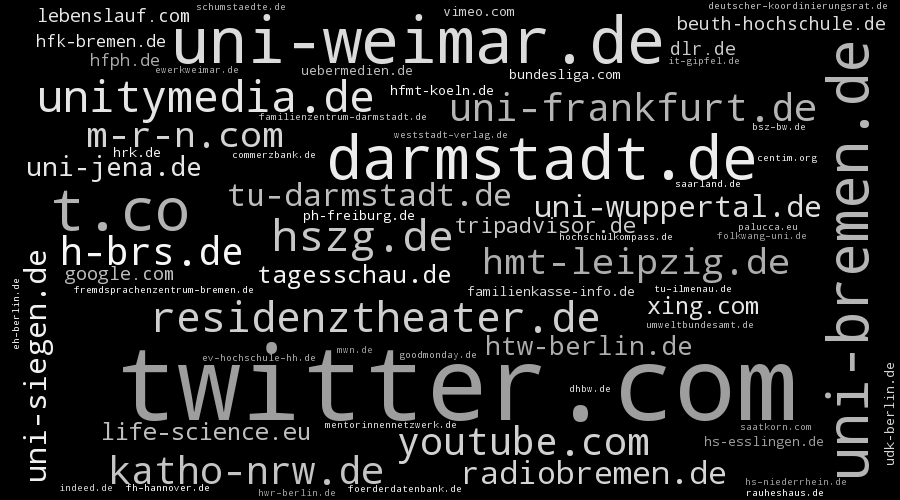
\includegraphics[width=\columnwidth, height=180pt]{../aufg02/wordcloud}	
	
  \end{frame}	
	
	
  \begin{comment}

  % Afrika und die Tropen 1
  \begin{frame}
    \frametitle{Die Tropen und Afrika (I)}
    \includegraphics[width=\textwidth]{pix/poverty}\\
    \begin{tiny}
Quelle: World Malaria Report 2014, World Health Organization, Markierungen der Breiten ergänzt
    \end{tiny}
  \end{frame}
  
  % Afrika und die Tropen 2
  \begin{frame}
    \frametitle{Die Tropen und Afrika (II)}
    
    \includegraphics[height=0.95\textheight,width=0.5\textwidth]{pix/gdp_per_capita}
    \includegraphics[width=0.5\textwidth]{pix/poverty_africa_europe}\\
    \begin{tiny}
Quelle: Bloom, Sachs, u.a., Geography, Demography, and Economic Growth in Africa, S. 217, Zahlen von 1995
    \end{tiny}
  \end{frame}
  
  % Landwirtschaft
  \begin{frame}
    \frametitle{Klima \& Landwirtschaft}
    \includegraphics[height=\textheight]{pix/africa_satellite}
    %\includegraphics[width=0.95\textwidth]{pix/pop_density}\\
    \begin{tiny}
Quelle: NASA, http://visibleearth.nasa.gov/view.php?id=57752 18.04.2016
%Quelle: Bloom, Sachs, u.a., Geography, Demography, and Economic Growth in Africa, S. 217
  \end{tiny}
  \end{frame}
  
  \begin{frame}
    \frametitle{Malaria}
    \includegraphics[width=\textwidth]{pix/malaria}\\
    \begin{tiny}
     
Quelle: World Malaria Report 2014, World Health Organization
    \end{tiny}
  \end{frame}
  
  %\begin{frame}
  %  \frametitle{AIDS}
  %\end{frame}
  
  \begin{frame}
    \frametitle{Hürden für Transport und Handel}
    
    \includegraphics[height=\textheight]{pix/africa_topo}
    \begin{tiny}
    http://photojournal.jpl.nasa.gov/jpegMod/PIA04965\_modest.jpg, 18.04.2016
    \end{tiny}
  \end{frame}
  
  \begin{frame}
   \frametitle{Zusammenfassung}
   \begin{itemize}
    \item Armut in den Tropen und Afrika
    \item Klima und Landwirtschaft
    \item Krankheiten
    \item Hürden für Transport und Handel
   \end{itemize}

  \end{frame}
  
  \begin{frame}
    \frametitle{Demographische Entwicklung}
    \includegraphics[width=0.9\textwidth,height=0.9\textheight]{pix/africas_share_of_world_income_and_population}\\
    \begin{tiny}
Quelle: Bloom, Sachs, u.a., Geography, Demography, and Economic Growth in Africa, S. 241
    \end{tiny}
  \end{frame}
  
  \begin{frame}
    \frametitle{Bevölkerungsverteilung \& Bevölkerungsdichte}
    \includegraphics[width=0.9\textwidth,height=0.9\textheight]{pix/pop_density}\\
    \begin{tiny}
Quelle: Bloom, Sachs, u.a., Geography, Demography, and Economic Growth in Africa, S. 217
    \end{tiny}
  \end{frame}
  
  \begin{frame}
    \frametitle{HIV Infektionen}
    \includegraphics[width=0.9\textwidth,height=0.9\textheight]{pix/HIV_all_2013}\\
    \begin{tiny}
Quelle: Global health sector response to HIV, 2000-2015, WHO
    \end{tiny}
  \end{frame}
  
  \begin{frame}
    \frametitle{Tote durch HIV}
    \includegraphics[width=0.9\textwidth,height=0.9\textheight]{pix/aids_tote_global_health_sector_response_to_hiv}\\
    \begin{tiny}
Quelle: Global health sector response to HIV, 2000-2015, WHO
    \end{tiny}
  \end{frame}

  \end{comment}
  
  %\begin{frame}
   % \frametitle{Quellen}
    
    %\printbibliography
  %\end{frame}

% etc
\end{document}